
%%%%%%%%%%%%%%%%%%%% author.tex %%%%%%%%%%%%%%%%%%%%%%%%%%%%%%%%%%%
%
% sample root file for your "contribution" to a contributed volume
%
% Use this file as a template for your own input.
%
%%%%%%%%%%%%%%%% Springer %%%%%%%%%%%%%%%%%%%%%%%%%%%%%%%%%%


% RECOMMENDED %%%%%%%%%%%%%%%%%%%%%%%%%%%%%%%%%%%%%%%%%%%%%%%%%%%
\documentclass[graybox,a4paper]{svmult}

% choose options for [] as required from the list
% in the Reference Guide

\usepackage{mathptmx}       % selects Times Roman as basic font
\usepackage{helvet}         % selects Helvetica as sans-serif font
\usepackage{courier}        % selects Courier as typewriter font
\usepackage{type1cm}        % activate if the above 3 fonts are
                            % not available on your system
%
\usepackage{makeidx}         % allows index generation
\usepackage{wrapfig}
\usepackage{graphicx}        % standard LaTeX graphics tool
                             % when including figure files
\usepackage{multicol}        % used for the two-column index
\usepackage[bottom]{footmisc}% places footnotes at page bottom
\usepackage{marginnote}
\newcommand{\TODO}[1]{\marginnote{TODO: #1}}    % TODO Befehl
\usepackage{units,amsmath}
\usepackage{todonotes}
\usepackage{hyperref}
\hypersetup{
    colorlinks=true,
    linkcolor=blue,
    filecolor=magenta,      
    urlcolor=cyan,
}
\usepackage{url}
\usepackage{siunitx}
\usepackage{units}
\usepackage{subcaption}
% see the list of further useful packages
% in the Reference Guide

\makeindex             % used for the subject index
                       % please use the style svind.ist with
                       % your makeindex program

%\usepackage{cleveref}[2012/02/15]
%\crefformat{footnote}{#2\footnotemark[#1]#3}

\renewcommand{\O}{{\cal O}}
\renewcommand{\leadsto}{\rightsquigarrow}
\newcommand{\V}[1]{\text{\boldmath $#1$}}    % Format for "Vector"
\newcommand{\M}[1]{\V{#1}}                   % Format for "Matrix"

\newcommand{\R}{\mathbbm{R}}                 % set of real number
\newcommand{\N}{\mathbbm{N}}                 % set of natural numbers
\newcommand{\C}{\mathbbm{C}}                 % ...
\newcommand{\1}{\mathbbm{1}}                 % identity matrix


%%%%%%%%%%%%%%%%%%%%%%%%%%%%%%%%%%%%%%%%%%%%%%%%%%%%%%%%%%%%%%%%%%%%%%%%%%%%%%%%%%%%%%%%%

%%
% Motivation, Problem Statement, Related Work (one page)
% Technical Approach (one page)
% Results (one page)
% Experiments completed or scheduled (one page)
% Main experimental insights (one page)
% References (one page)
%%

\begin{document}

\title*{L.U.N.A. - A Laser-Mapping Unidirectional Navigation Actuator} 
\author{Jasper Zevering, Anton Bredenbeck, Fabian Arzberger,
  Dorit Borrmann and Andreas N\"uchter}
% FIXME sort the authors
% Use \authorrunning{Short Title} for an abbreviated version of
% your contribution title if the original one is too long
\institute{All authors are with Informatics VII -- Robotics and
  Telematics, University of W\"urzburg, Am Hubland, 97074 W\"urzburg
  \email{borrmann@informatik.uni-wuerzburg.de %\\|  \email{jasper.zevering@stud-mail.uni-wuerzburg.de} \\ | \email{anton.bredenbeck@stud-mail.uni-wuerzburg.de}\\ |  \email{fabian.arzberger@stud-mail.uni-wuerzburg.de
  }
%\and Name of Second Author \at Name, Address of Institute 
%\email{name@email.address}
}
%
% Use the package "url.sty" to avoid
% problems with special characters
% used in your e-mail or web address
%
\maketitle

%\abstract*{Each chapter should be preceded by an abstract (10--15 lines long) 
%that summarizes the content. The abstract will appear \textit{online} at 
%\url{www.SpringerLink.com} and be available with unrestricted access. This 
%allows unregistered users to read the abstract as a teaser for the complete 
%chapter. As a general rule the abstracts will not appear in the printed 
%version 
%of your book unless it is the style of your particular book or that of the 
%series to which your book belongs.
%Please use the 'starred' version of the new Springer \texttt{abstract} command 
%for typesetting the text of the online abstracts (cf. source file of this 
%chapter template \texttt{abstract}) and include them with the source files of 
%your manuscript. Use the plain \texttt{abstract} command if the abstract is 
%also to appear in the printed version of the book.}

\abstract{
This paper proposes an autonomous approach to 3D mapping using the concept of impulse by  conservation of angular momentum (IBCOAM) as a unidirectional drive to roll a 2D laser scanner in an IMU equipped, pose-tracked spherical robot system.
An experimental prototype of the robot is introduced, giving details about the hardware.
The laser scanning results as well as the IBCOAM drive data that have been gathered using the prototype are analyzed, revealing  technical challenges.
}

\section{Introduction}
\label{sec:introduction}

In today's world, autonomous robots have found their way into everyday life in a variety of ways. 
This includes, but is not limited to, the vacuum cleaner that independently navigates one's living-room or mobile robots employed for exploration of areas that are too dangerous for humans.
To foster new advances in the latter, specifically for underground environments, the  Defense Advanced Research Projects Agency (DARPA) of the US Defense Department established the yearly ``SubT'' Challenge in 2017.
In this challenge, teams are tasked to ``Drive novel approaches and technologies to allow warfighters and first-responders to rapidly map, navigate, and search dynamic underground environments.''~\cite{allen} proving the demand for further research in this domain.
One subtask of this challenge is building an accurate 3D model of the environment, i.e., mapping the surroundings. 
This paper shows a proof of concept of a such a novel approach and validates it with experiments.

One such approach using a 2D laser scanner to scan 3D indoor environments has been proposed in~\cite{classical_mechanics_scanner}.
The authors mount a 2D laser scanner on a cylindrical structure.
An operator then initiates a rolling motion by manually pushing the contraption.
This enables the scanner to sense the 3D environment successfully.
However, manually pushing the scanner is not practical, especially for long scans.

Previous work includes our RADLER (RADial LasER scanning device), which consists of a 2D laser scanner attached to the axle of a unicycle~\cite{ISER2018}.
An operator pushes the unicycle along a requested path.
The inherent rotation of the wheel creates a radial 3D laser scanning pattern.
However, this approach still requires an operator, therefore does not fulfill the autonomy requirements. 

A more autonomous approach was taken by Fang et al.~\cite{3D_per_2D_based}.
The authors mounted a rotating 2D laser-scanner on top of a turtle-bot thus removing the need of an operator.
In contrast to the RADLER however, the turtle-bot does not provide an inherent rotation.
Therefore an additional actuator is required to create the radial 3D scanning-pattern. 

This paper builds upon the results of the RADLER and has a specific application of mapping lunar craters autonomously in mind.
We propose a novel approach to low-cost 3D laser scanning using a 2D laser scanner inside a spherical robot based on conversation of angular momentum (COAM): the L.U.N.A. - sphere (Laser-mapping Unidirectional Navigation Actuator).
The 2D laser scanner is fixed to the spherical structure, hence a similar situation as with the RADLER is given: the inherent rotation of the sphere creates a radial 3D scanning pattern.
Using the format of a spherical robot permits the system to be designed more compact. 
Additionally, the spherical shell doubles as a protective layer for the actuators, sensors and electronics. 
This is especially valuable for applications in rough terrain or scenarios in which non-minimal impact is expected, such as space applications.
During a launch, withstanding large G-forces is a necessary requirement, which can be better implemented using the spherical format. 
Furthermore, an operator is no longer required given a drive implemented in the robot.


\section{State of the Art}
\label{sec:stateOfTheArt}
As evolution of RADLER, a hand-driven radial scanner device, a self-driving spherical approach was chosen to ensure robustness and autonomy.  There have been several works in literature regarding approaches for spherical robots, of which an overview will be given in the following. 

\subsection{Spherical Robots}
\label{sec:stateOfTheArt:sphericalrobots}
An early idea of an self-driving sphere has been introduced by J.L. Tate in 1893 who claimed the patent  508 and 558 in  the U.S. for a sphere, driven by an inner moving counterweight, which got its torque from an spring. This idea of an actuator attached to an counterweight pointing to the bottom and therefore the torque being transferred to the sphere and moving it, is still a widespread approach for spherical robots.

In \cite{soa1} a basic motion control system for the BYQ-III is introduced. The BYQ-III has a mass of 25kg and a diameter of 600mm and its driving mechanism has been proposed in \cite{soa2} by S.Hanxu, X,Aiping, J.Qingxuan and W.Liangqing. It contains  a counterweight pendulum, four gyro actuators, providing movement for two axes and one IMU mounted on the gyros' case. There is no extra payload or sensor, nor would there be space for a centered measurement unit due to the centered counterweight. Therefore the counterweight leads to a steady movement, not relying on acceleration but on velocity of the actuators and therefore providing continuous speed.

A second spherical robot with its driving mechanism relaying on inner counterweight is presented in \cite{soa3}. This robot was designed for movement on a water surface and therefore has fins mounted to the shell orthogonal to the movement. Two actuators attached to the shell and the inner counterweight provide movement around one axis. In contrast to the BYQ-III a middle-centered  sensor would be possible, but this would have no movement relative to the surface, as it would be part of the relatively non moving inner counterweight. It also has steady, well controllable movement. 
The spheres presented in \cite{soa4} and \cite{soa5} provide a solution for a driving system which does not rely on a moving inner counterweight but uses internal reaction wheels to provide torque. This leads to theoretically having middle-centered space available, which would be rotating with respect to the surface. However, the prototype provided by V. Muralidharan et al. shows less controllability then counterweight driven spheres. Furthermore, this robot is driven by acceleration and not velocity which leads to limited movement capabilities.

A third approach for spherical robots relys on an internal unit which drives inside the sphere. A Design and control approach is provided in \cite{soa6} where a four-wheeled vehicle moves in the sphere to initiate rolling by moving the center of mass in the desired direction. This technical solution is capable of a nearly maximum size of possible payload in relation to the overall-size, but also does not provide a rotation of the sensor which would be needed for 3D laser scanning. Additionally, this provides good controllability, similar to the the counterweight driven approach. It is obviously not as stable regarding external perturbations or forces, as there is no fixed connection to the shell. This would make it not suitable for missions with extreme forces and unknown starting conditions like missions involving a rocket launch or a hard landing to get to the starting point. In a worst case scenario this could lead to a start with the unit being rotated by 180 degrees and therefore not being able to bring torque to the sphere. A similar situation could occur if the sphere was stuck to the environment and therefore the inner unit would try to perform a whole revolution (``looping'') inside the sphere, which would cause the car to fall on its back, i.e. a supine position.

Overcoming this shortage of the inner unit just relying on gravity to apply its force to the shell, \cite{soa7} introduced the approach of a rod, expanded by a spring to the maximum possible size and having a wheel on one side. The wheel generates the movement by also moving the center of mass. However, now the non-reversible supine position does not exist anymore. Even with the wheel at the top, it is still pressed to the shell by the spring and therefore is capable of maintaining its movement. Again this approach does not provide spin of a centered  placed sensor without further contraptions.


\section{Technical Approach}
\label{sec:TechnicalApproach}

\begin{figure}
\centering
\begin{subfigure}[b]{0.64\textwidth}
        \centering
        \includegraphics[width=\textwidth]{../Media/sphere_fullshell_left.jpg}
        \caption{Hardware setup of the L.U.N.A sphere prototype, including notches in the shell and friction granule.}
        \label{sec:TechnicalApproach:fig:prototype}
\end{subfigure}
\hfill
\begin{subfigure}[b]{0.34\textwidth}
        \centering
        \includegraphics[width=\textwidth]{../Media/sphere_right_motor.jpg}
        \caption{IMU (beneath supporting structure) and brushless motor (above supporting structure) of the L.U.N.A sphere without shell, including flywheel mass. }
        \label{sec:TechnicalApproach:fig:motor}
\end{subfigure}
\\
\caption{Hardware setup of the L.U.N.A sphere prototype, including notches in the shell and friction granule.}
\end{figure}

Figure \ref{sec:TechnicalApproach:fig:prototype} shows the final hardware setup of the robot. In order to reduce complexity with respect to the 3D-transformation calculations, the laserscanner was placed at the center of a spherical acrylic glass shell as close as possible. This limits the laser scanners movement to rotational movement and removes translational movement completely. With this initial setup given the only room left for the acrylic glass structural components, batteries, boardcomputer, IMUs, motors, weights and wiring are the spacings between the scanner and the shell. Figure \ref{sec:TechnicalApproach:fig:motor} shows one 
\todo[inline]{Insert motor name (data sheet reference?)}
motor of the COAM drive with two flywheels attatched. Strong epoxy glue attaches the weights to the motor shafts. As the flywheels start spinning with respect to the structural components of the sphere, the sphere itself starts spinning with respect to the ground. 

\subsection{Hardware Setup}
\label{sec:TechnicalApproach:HardwareSetup}

Figure \ref{sec:TechnicalApproach:fig:prototype} also shows that the top and the bottom of the shell are covered in salt, which made a good granule to increase friction to the ground in the early testing phase. Furthermore, there are notches in the front side of the shell to increase permeability for the laser. Unfortunately, the laser scanner measurements are still very much affected by blockades due to components of the sphere. Specifically, the outside shell is a strongly inhibiting factor as an object with the distance of the radius is measured at all times.
                                                                                                                                                                                                                  
\begin{figure}                                                                                                                                                                                                    
\centering                                                                                                                                                                                                        
\includegraphics[width=\textwidth]{../Media/BlueprintPNG.png}                                                                                                                                                      
\caption{Blueprint that shows the mechanical structure of the spherical robot.}                                                                                                                                   
\label{sec:TechnicalApproach:fig:blueprint}                                                                                                                                                                       
\end{figure}                                                                                                                                                                                                      
                                                                                                                                                                                                                  
Figure \ref{sec:TechnicalApproach:fig:blueprint} shows a CAD blueprint about the rough interior layout of the mechanical structure of the L.U.N.A sphere, ignoring flyweights and wiring. The blueprint shows that the payload is mounted to supporting structural components which are made of acrylic glass. The raspberry pi model 3 boardcomputer is placed on top of the laser. Above that, another supporting structure can hold additional counterweights to correct for unhomogeneous weight distribution or an off place center of mass.                                                                                                     
The battery finds its place in front of the laserscanner on another supporting structure. The two brushless motors were each placed on one side of the supporting structure with spacers that leave room for the side IMU underneath one of the motors. Two other IMUs are placed in front of and beneath the laser to ensure coverage of all axes.                                                                                 
                                                                                                                                                                                                                  
\subsection{Sensor Integration}                                                                                                                                                                                   
\label{sec:TechnicalApproach:SensorIntegration}

\begin{figure}                                                                                                                                                                                                    
\centering
%\includegraphics[width=0.5\textwidth]{./photo/imuvirtual.png}                                                                                                                                                      
\caption{Sketch that helps illustrate the combination of 3 IMUs into 1 virtual IMU that simulates being in the center of the sphere.}                                                                                                                           
\label{sec:SensorIntegration:fig:virtual}                                                                                                                                                                       
\end{figure}                                                                                                                                                                                                      

The sensor integration was fully implemented with the Robot Operating System (ROS) that has been installed on a default ubunty running on a rasperry pi 3.
Overall, three seperate PhidgetsSpacial 10441B IMUs \cite{imuphidgets} have been used to keep track of the spheres pose. Figure \ref{sec:SensorIntegration:fig:virtual} helps illustrate why three IMUs are used instead of just one. A previous study has shown that transforming the data of only one non-centered IMU leads to less quality measurements. However, combining the measurements of three IMUs, where each of which measures only the static rotation around one of their rotation axis (which also represents a rotation axis of the sphere), leads to better results. Each IMU is perpendicular to the other two, so combining the axis measurements leads to a "virtual" IMU, that simulates beeing an IMU that takes measurements from the middle of the sphere, making precise rotation speed measurements possible. 

The IMUs also ship with accelerometers that are used to determine the full pose of the sphere. Each IMU calculates their pose seperatly, using a quaternion extended kalman filter (QEKF). However, combining those poses into one did not have any positive effect, but only made the software more resource demanding and slow. Thats why only the pose of the bottom IMUs accelerometers are used to keep track of the pose.

The motors have first been accessed with the wiringPi library for raspberry pi. This library may seemed like a good prototyping library with fast results, but a switch to the more advanced piGPIO library allowed a higher throttle resolution. 

Unfortunately, the brass weights were not drilled in the very center, causing an imbalance when rotating. The resulting vibrations inhibit the movement of the sphere thus a controller was implemented that measures the extent of the vibrations using standard deviations of the IMUs axis that are not rolled over and adjusts the throttle of the motors accordingly. This was done with a simple two-point controller with hysteresis which already leads to satisfying results. The second approach of a PID controller for not letting the vibrations getting beyond the upper threshold of the hysteresis controller failed because no satisfying method of differing the normal vibrations during rolling from vibrations which leads to stopping by slipping was found. Considering the velocity of the sphere is not possible, because the speed of the sphere is calculated by the rotating speed and therefore slip of the sphere does not detect translational deceleration. 





\section{Experimental Results}
\label{sec:experimentalResults}


\subsection{3D Laser Scanning}
\label{sec:experimentalResults:3DLaserScanning}



\subsection{COAM Drive}
\label{sec:experimentalResults:COAMDrive}

\begin{figure}
\centering
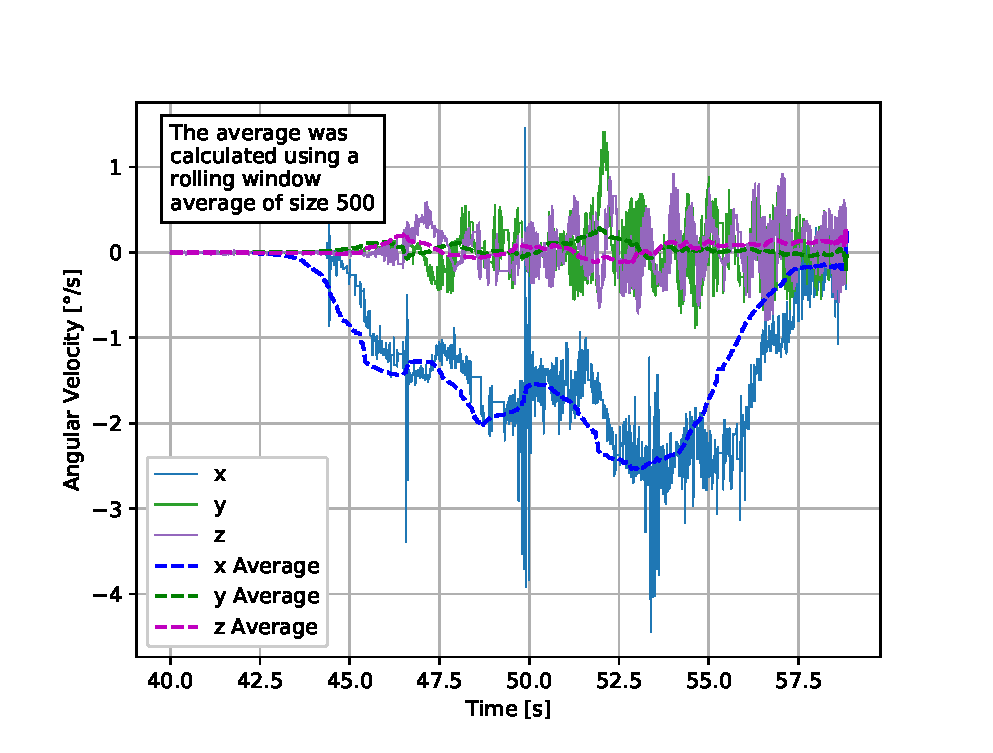
\includegraphics[width=\textwidth]{./plotsAndScripts/angVel-2020-01-29-16-14-54/ang-vel}
\caption{Angular velocities of the L.U.N.A. - sphere during a test run. The flywheels rotate around the x-axis in positive direction. Velocities in the other direction can mostly be contributed to vibrations and tilt of the robot.}
\label{sec:experimentalResults:COAMDrive:fig:angvel}
\end{figure}

\section{Conclusions}
\label{sec:conclusions}

\todo[inline]{Add conclusion}

\begin{acknowledgement}
The authors thank Dieter Ziegler and Sergio Montenegro for supporting our work. We acknowledge funding from the ESA Contract No. 4000130925/20/NL/GLC for the ``DAEDALUS -- Descent And Exploration in Deep Autonomy of Lava Underground Structures'' Open Space Innovation Platform (OSIP) lunar caves-system study and the Elite Network Bavaria (ENB) for providing funds for the academic program ``Satellite Technology''.

\bigskip

\noindent \textbf{Authors Note}
In an attempt to abide by the \href{https://www.go-fair.org/fair-principles}{Fair-Principles} of open science the authors provided all code developed and further information at their \href{https://github.com/fallow24/L.U.N.A}{GitHub} page.
\end{acknowledgement}

\bibliographystyle{plain}
\bibliography{andreas_publications}

\end{document}
